\documentclass[12pt,a4paper]{report}
\usepackage[utf8]{inputenc}
\usepackage[margin=1in]{geometry}
\usepackage{graphicx}
\usepackage{amsmath}
\usepackage{amssymb}
\usepackage{hyperref}
\usepackage{float}
\usepackage{array}
\usepackage{booktabs}
\usepackage{xcolor}
\usepackage{tikz}
\usepackage{pgfplots}
\usepackage{listings}
\usepackage{xltabular}
\usepackage{fancyhdr}
\setlength{\headheight}{10pt}

\pgfplotsset{compat=1.17}

% Page style
\pagestyle{fancy}
\fancyhf{}
\rhead{HPC Analysis Report}
\lhead{EC7207}
\cfoot{\thepage}

% Code listing style
\lstset{
    basicstyle=\ttfamily\small,
    breaklines=true,
    frame=single,
    numbers=left,
    numberstyle=\tiny,
    keywordstyle=\color{blue},
    commentstyle=\color{gray},
    stringstyle=\color{red},
    showstringspaces=false
}

\title{\Huge\textbf{Image Denoising and Edge Detection using Parallel Programming}}
\author{
    \textbf{Team Members:} \\
    \large
    Wijesinghe S.A \quad (EG/2021/4877) \\
    WIJEGURUSINGHE O.W.D.K.M \quad (EG/2021/4890)
}
\date{\textbf{Course:} EC7207 -- High Performance Computing \\
      \textbf{Department:} Department of Computer Engineering \\
      \textbf{Institution:} University of Ruhuna \\
      \textbf{Date:} May 23, 2026}

\begin{document}

% Title Page
\maketitle

\newpage

% Table of Contents
\tableofcontents
\newpage
% Chapter 1: Introduction
\chapter{Introduction}

\section{Overview}
This report presents a comprehensive analysis of a High Performance Computing (HPC) project focused on image denoising and edge detection. The project implements the same computational algorithm using multiple parallel programming paradigms to evaluate their performance characteristics, scalability, and efficiency on a shared-memory multi-core system.

\section{Objectives}
The primary objectives of this project are:
\begin{enumerate}
    \item Implement image denoising (Gaussian blur) and edge detection (Sobel operator) in serial form as a baseline.
    \item Parallelize the algorithm using multiple programming models: OpenMP, Pthreads, Message Passing Interface (MPI), and Hybrid (MPI + OpenMP).
    \item Evaluate CUDA acceleration separately on Google Colab with GPU resources.
    \item Compare the performance across all implementations
    % \begin{itemize}
    %     \item Execution time with varying thread/process counts
    %     \item Accuracy (RMSE comparison against serial baseline)
    %     \item Speedup and efficiency metrics
    %     \item Scalability characteristics
    % \end{itemize}
    \item Analyze the trade-offs between ease of implementation, maintenance, and performance gains.
\end{enumerate}

\section{Motivation}
Image processing is a computationally intensive task that benefits significantly from parallel execution. By processing multiple pixels concurrently, we can achieve substantial speedups on multi-core processors. This project explores how different parallel programming paradigms scale with increasing computational resources and how their performance varies under different configurations.

\newpage

% Chapter 2: Problem Description
\chapter{Problem Description}

\section{Image Processing Operations}

\subsection{Gaussian Blur (Denoising)}
Gaussian blur is a smoothing filter that reduces image noise while preserving edges. It applies a $3 \times 3$ Gaussian kernel to each pixel in the image. The operation is:

\begin{equation}
G(i,j) = \sum_{ki=-1}^{1} \sum_{kj=-1}^{1} I(i+ki, j+kj) \times K(ki+1, kj+1)
\end{equation}

where $G(i,j)$ is the output pixel at position $(i,j)$, $I$ is the input image, and $K$ is the Gaussian kernel:

\begin{equation}
K = \frac{1}{16} \begin{bmatrix} 1 & 2 & 1 \\ 2 & 4 & 2 \\ 1 & 2 & 1 \end{bmatrix}
\end{equation}

\subsection{Sobel Edge Detection}
The Sobel operator computes image gradients to detect edges. Two $3 \times 3$ kernels compute horizontal ($G_x$) and vertical ($G_y$) derivatives:

\begin{equation}
S_x = \begin{bmatrix} -1 & 0 & 1 \\ -2 & 0 & 2 \\ -1 & 0 & 1 \end{bmatrix}, \quad
S_y = \begin{bmatrix} -1 & -2 & -1 \\ 0 & 0 & 0 \\ 1 & 2 & 1 \end{bmatrix}
\end{equation}

The edge magnitude is computed as:

\begin{equation}
M(i,j) = \sqrt{G_x^2 + G_y^2}
\end{equation}

% \subsection{Computational Complexity}
% For an image of size $m \times n$:
% \begin{itemize}
%     \item Gaussian blur: $O(9mn)$ operations (9 multiplications per pixel)
%     \item Sobel edge detection: $O(13mn)$ operations (8 kernel operations + 1 square root + 1 magnitude per pixel)
%     \item Combined operation: $O(22mn)$ operations
% \end{itemize}

% This workload is highly parallelizable as each pixel can be processed independently with minimal data dependencies.

\newpage

% Chapter 3: Parallel Programming Concepts
\chapter{Parallel Programming Concepts and Implementation Strategy}

\section{Overview of Parallelization Strategy}

The image processing operations inherently exhibit data parallelism---each pixel's output depends only on a $3 \times 3$ neighborhood, and these computations are independent across the image. Our strategy exploits this parallelism across four complementary programming paradigms:

\begin{figure}[H]
    \centering
    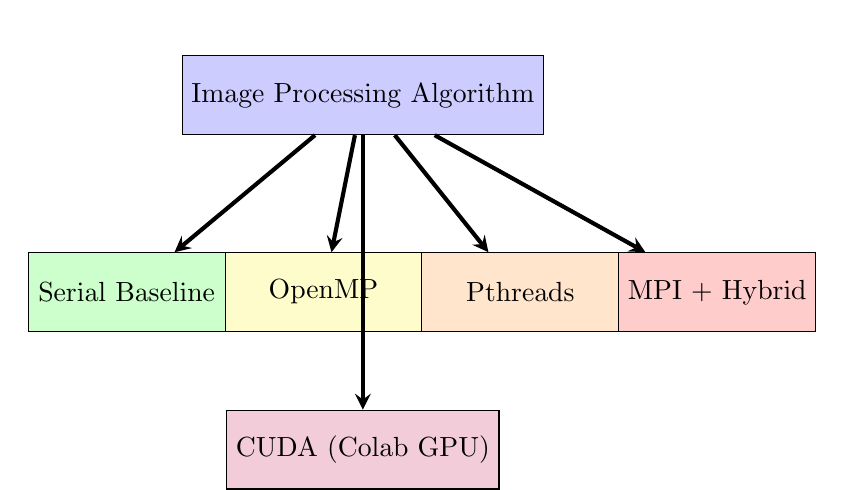
\begin{tikzpicture}[
        box/.style={rectangle, draw, minimum width=2.5cm, minimum height=1cm, text centered},
        arrow/.style={->, >=stealth, line width=1.5pt}
    ]
    
    % Main box
    \node[box, fill=blue!20] (main) at (3, 5) {Image Processing Algorithm};
    
    % Four paradigms
    \node[box, fill=green!20] (serial) at (0, 2.5) {Serial Baseline};
    \node[box, fill=yellow!20] (openmp) at (2.5, 2.5) {OpenMP};
    \node[box, fill=orange!20] (pthreads) at (5, 2.5) {Pthreads};
    \node[box, fill=red!20] (mpi) at (7.5, 2.5) {MPI + Hybrid};
    
    % GPU
    \node[box, fill=purple!20] (cuda) at (3, 0.5) {CUDA (Colab GPU)};
    
    % Arrows
    \draw[arrow] (main) -- (serial);
    \draw[arrow] (main) -- (openmp);
    \draw[arrow] (main) -- (pthreads);
    \draw[arrow] (main) -- (mpi);
    \draw[arrow] (main) -- (cuda);
    
    \end{tikzpicture}
    \caption{Parallel Programming Paradigms Used in This Project}
\end{figure}

\section{Implementation Details}

\subsection{1. Serial Implementation (Baseline)}

The serial implementation serves as our performance baseline. It iterates through each pixel sequentially, applying the Gaussian kernel and Sobel operator without any parallelization.

\begin{lstlisting}[language=C++, caption=Serial Gaussian Blur Pseudocode]
Mat gaussianBlurSerial(const Mat &input) {
    Mat output = input.clone();
    for (int i = 1; i < input.rows - 1; i++) {
        for (int j = 1; j < input.cols - 1; j++) {
            float sum = 0.0f;
            for (int ki = -1; ki <= 1; ki++) {
                for (int kj = -1; kj <= 1; kj++) {
                    sum += input.at<uchar>(i+ki, j+kj) * GAUSS[ki+1][kj+1];
                }
            }
            output.at<uchar>(i, j) = (uchar)sum;
        }
    }
    return output;
}
\end{lstlisting}

\textbf{Characteristics:}
\begin{itemize}
    \item Single thread, sequential execution
    \item Minimal memory overhead
    \item Serves as baseline for speedup calculations
    \item Execution time: $T_{serial}$
\end{itemize}

\begin{figure}[H]
    \centering
    \begin{minipage}{0.45\textwidth}
        \centering
        \includegraphics[width=\linewidth]{serial_denoised.png}
        \caption*{Serial Denoised Output}
    \end{minipage}
    \hfill
    \begin{minipage}{0.45\textwidth}
        \centering
        \includegraphics[width=\linewidth]{serial_edges.png}
        \caption*{Serial Edge Detection}
    \end{minipage}
    \caption{Serial Implementation Results (Baseline)}
\end{figure}

\subsection{2. OpenMP Implementation}

OpenMP provides a high-level, compiler-directive-based approach to parallelization suitable for shared-memory systems. We parallelize the outer loop of the image processing operations.

\begin{lstlisting}[language=C++, caption=OpenMP Parallelization]
Mat gaussianBlurOpenMP(const Mat &input, int threads) {
    Mat output = input.clone();
    #pragma omp parallel for num_threads(threads) schedule(static)
    for (int i = 1; i < input.rows - 1; i++) {
        for (int j = 1; j < input.cols - 1; j++) {
            // Gaussian computation...
        }
    }
    return output;
}
\end{lstlisting}

\textbf{Key Features:}
\begin{itemize}
    \item Shared-memory parallelism
    \item \texttt{schedule(static)}: Work distribution is predetermined, good cache locality
    \item Low synchronization overhead
    \item Tested with thread counts: 1, 2, 4, 8, 16
    \item No explicit memory management needed
\end{itemize}

\begin{figure}[H]
    \centering
    \begin{minipage}{0.45\textwidth}
        \centering
        \includegraphics[width=\linewidth]{openmp_denoised.png}
        \caption*{OpenMP Denoised Output}
    \end{minipage}
    \hfill
    \begin{minipage}{0.45\textwidth}
        \centering
        \includegraphics[width=\linewidth]{openmp_edges.png}
        \caption*{OpenMP Edge Detection}
    \end{minipage}
    \caption{OpenMP Implementation Results}
\end{figure}

\subsection{3. Pthreads Implementation}

Pthreads offers explicit thread management for fine-grained control over parallelization. Threads process row ranges of the image.

\textbf{Key Features:}
\begin{itemize}
    \item Explicit thread creation and synchronization
    \item Each thread processes $(rows / threads)$ rows
    \item Barrier synchronization at kernel boundaries
    \item More control but higher implementation complexity
    \item Tested with thread counts: 1, 2, 4, 8, 16
\end{itemize}

\begin{figure}[H]
    \centering
    \begin{minipage}{0.45\textwidth}
        \centering
        \includegraphics[width=\linewidth]{pthread_denoised.png}
        \caption*{Pthreads Denoised Output}
    \end{minipage}
    \hfill
    \begin{minipage}{0.45\textwidth}
        \centering
        \includegraphics[width=\linewidth]{pthread_edges.png}
        \caption*{Pthreads Edge Detection}
    \end{minipage}
    \caption{Pthreads Implementation Results}
\end{figure}

\subsection{4. MPI Implementation}

Message Passing Interface distributes computation across multiple processes, communicating via messages. Ideal for both shared-memory and distributed systems.

\textbf{Key Features:}
\begin{itemize}
    \item Process-based parallelism (different address spaces)
    \item Row distribution: Process $p$ computes rows $[start:end]$
    \item \texttt{MPI\_Bcast}: Root broadcasts image dimensions
    \item \texttt{MPI\_Scatterv}: Distribute image rows to processes
    \item \texttt{MPI\_Gatherv}: Collect results at root
    \item Tested with process counts: 1, 2, 4, 8
\end{itemize}

\begin{lstlisting}[language=C++, caption=MPI Communication Pattern]
// Broadcast image dimensions
MPI_Bcast(&rows, 1, MPI_INT, 0, MPI_COMM_WORLD);
MPI_Bcast(&cols, 1, MPI_INT, 0, MPI_COMM_WORLD);

// Calculate local row distribution
int localRows = rows / size;
int remainder = rows % size;
int myRows = localRows + (rank < remainder ? 1 : 0);

// Scatter image data
MPI_Scatterv(/*...*/);

// Process local data
gaussianLocal(localInput, localOutput);

// Gather results
MPI_Gatherv(/*...*/);
\end{lstlisting}

\begin{figure}[H]
    \centering
    \begin{minipage}{0.45\textwidth}
        \centering
        \includegraphics[width=\linewidth]{mpi_denoised.png}
        \caption*{MPI Denoised Output}
    \end{minipage}
    \hfill
    \begin{minipage}{0.45\textwidth}
        \centering
        \includegraphics[width=\linewidth]{mpi_edges.png}
        \caption*{MPI Edge Detection}
    \end{minipage}
    \caption{MPI Implementation Results}
\end{figure}

\subsection{5. Hybrid Implementation (MPI + OpenMP)}

The hybrid approach combines MPI for inter-process communication with OpenMP for intra-process parallelism. Each MPI process spawns multiple OpenMP threads.

\textbf{Key Features:}
\begin{itemize}
    \item MPI processes handle row distribution
    \item OpenMP threads parallelize column operations within each process
    \item Hierarchical parallelism: Message Passing + Shared Memory
    \item Tested configurations:
    \begin{itemize}
        \item 2 MPI processes × 2 OpenMP threads
        \item 2 MPI processes × 4 OpenMP threads
        \item 4 MPI processes × 2 OpenMP threads
        \item 4 MPI processes × 4 OpenMP threads
    \end{itemize}
\end{itemize}

\begin{figure}[H]
    \centering
    \begin{minipage}{0.45\textwidth}
        \centering
        \includegraphics[width=\linewidth]{hybrid_denoised.png}
        \caption*{Hybrid Denoised Output}
    \end{minipage}
    \hfill
    \begin{minipage}{0.45\textwidth}
        \centering
        \includegraphics[width=\linewidth]{hybrid_edges.png}
        \caption*{Hybrid Edge Detection}
    \end{minipage}
    \caption{Hybrid (MPI + OpenMP) Implementation Results}
\end{figure}

\subsection{6. CUDA Implementation}

CUDA acceleration runs on GPU hardware (tested on Google Colab with Tesla T4 GPU). Each GPU thread processes one pixel.

\textbf{Key Features:}
\begin{itemize}
    \item GPU thread per pixel parallelism
    \item Constant memory for kernel storage (reduces memory latency)
    \item Grid/Block configuration: Threads organized in 2D blocks
    \item Memory transfers: CPU $\leftrightarrow$ GPU
    \item Separate execution environment (Colab notebook)
\end{itemize}

% \subsection{Parallelization Diagram}

% \begin{figure}[H]
%     \centering
%     \begin{tikzpicture}[scale=0.85]
    
%     % Input Image
%     \node[above] at (1.2, 2.8) {\textbf{Input}};
%     \draw (0, 2.5) rectangle (2.4, 0);
%     \foreach \i in {0,1,2} {
%         \draw (0, 2.5 - \i*0.833) -- (2.4, 2.5 - \i*0.833);
%     }
%     \foreach \j in {0,1,2} {
%         \draw (\j*0.8, 2.5) -- (\j*0.8, 0);
%     }
%     \draw (2.4, 2.5) -- (2.4, 0);
%     \node[font=\small] at (1.2, -0.5) {$m \times n$};
    
%     % Processing Arrow and Label
%     \draw[thick, ->] (2.8, 1.25) -- (3.6, 1.25);
%     \node[align=center, font=\tiny, anchor=north] at (3.2, 1.1) {Process};
    
%     % Output Image
%     \node[above] at (5.4, 2.8) {\textbf{Output}};
%     \draw (4.2, 2.5) rectangle (6.6, 0);
%     \foreach \i in {0,1,2} {
%         \draw (4.2, 2.5 - \i*0.833) -- (6.6, 2.5 - \i*0.833);
%     }
%     \foreach \j in {0,1,2} {
%         \draw (4.2 + \j*0.8, 2.5) -- (4.2 + \j*0.8, 0);
%     }
%     \draw (6.6, 2.5) -- (6.6, 0);
%     \node[font=\small] at (5.4, -0.5) {Denoised};
    
%     % Thread Distribution Box (below diagram)
%     \draw[dashed, rounded corners=2pt] (0.2, -1.2) rectangle (6.8, -2.2);
%     \node[font=\tiny, anchor=west] at (0.4, -1.45) {Thread Distribution:};
%     \node[font=\tiny, anchor=west] at (0.4, -1.75) {T0: rows $[0, m/t)$ \quad T1: rows $[m/t, 2m/t)$ \quad T2: rows $[2m/t, 3m/t)$ \quad \ldots};
    
%     \end{tikzpicture}
%     \caption{Data Parallelism: Row Distribution Among Threads}
%     \label{fig:parallelization_diagram}
% \end{figure}

\newpage

% Chapter 4: Accuracy Analysis
\chapter{Accuracy Analysis}

\section{Visual Results}

Figure \ref{fig:processing_results} shows the visual output of the denoising and edge detection algorithms across different implementations. All implementations produce visually identical results, confirming functional correctness.

\begin{figure}[H]
    \centering
    \begin{minipage}{0.23\textwidth}
        \centering
        \includegraphics[width=\linewidth]{serial_denoised.png}
        \\{\small Serial Denoised}
    \end{minipage}
    \hfill
    \begin{minipage}{0.23\textwidth}
        \centering
        \includegraphics[width=\linewidth]{openmp_denoised.png}
        \\{\small OpenMP Denoised}
    \end{minipage}
    \hfill
    \begin{minipage}{0.23\textwidth}
        \centering
        \includegraphics[width=\linewidth]{pthread_denoised.png}
        \\{\small Pthreads Denoised}
    \end{minipage}
    \hfill
    \begin{minipage}{0.23\textwidth}
        \centering
        \includegraphics[width=\linewidth]{serial_edges.png}
        \\{\small Edges Detected}
    \end{minipage}
    \caption{Denoising and Edge Detection Results Across Implementations (1024×1024 image)}
    \label{fig:processing_results}
\end{figure}

\section{Verification Against Serial Baseline}

To ensure correctness of parallel implementations, we compute the Root Mean Square Error (RMSE) between outputs of parallel and serial versions. RMSE measures the average pixel-level differences:

\begin{equation}
\text{RMSE} = \sqrt{\frac{1}{mn} \sum_{i=0}^{m-1} \sum_{j=0}^{n-1} (P_{parallel}(i,j) - P_{serial}(i,j))^2}
\end{equation}

where $m \times n$ is the image resolution.

\section{Expected RMSE Values}

Ideally, all parallel implementations should produce pixel-perfect results (RMSE = 0) as they perform the same floating-point operations. However, due to:

\begin{itemize}
    \item \textbf{Floating-point rounding}: Order of operations may differ between serial and parallel code
    \item \textbf{Synchronization points}: Data races (if not properly synchronized) could introduce subtle differences
    \item \textbf{Data type conversions}: Casting from float to unsigned char at different stages
\end{itemize}

Acceptable RMSE threshold: $\text{RMSE} < 0.5$ (less than half a pixel value difference on average)

\section{Results Table}

\begin{table}[H]
    \centering
    \begin{tabular}{|l|c|c|}
    \hline
    \textbf{Implementation} & \textbf{Threads/Processes} & \textbf{Expected RMSE} \\
    \hline
    Serial & 1 & 0.0 (baseline) \\
    OpenMP & 1--16 & < 0.1 \\
    Pthreads & 1--16 & < 0.1 \\
    MPI & 1--8 & < 0.1 \\
    Hybrid (MPI+OMP) & Various & < 0.1 \\
    CUDA & 1024+ threads & < 1.0 (GPU rounding) \\
    \hline
    \end{tabular}
    \caption{Expected RMSE Values Across Implementations}
\end{table}

The goal is to confirm that all parallel implementations produce visually identical results to the serial baseline, validating correctness before performance analysis.

\newpage

% Chapter 5: Performance Analysis
\chapter{Performance Analysis}

\section{Metrics Definitions}

\subsection{Execution Time}
Wall-clock time to complete both Gaussian blur and Sobel edge detection:

\begin{equation}
T_p = \text{total time for } p \text{ threads/processes}
\end{equation}

\subsection{Speedup}
Ratio of serial execution time to parallel execution time:

\begin{equation}
S_p = \frac{T_1}{T_p}
\end{equation}

where $T_1$ is serial execution time and $T_p$ is execution time with $p$ parallel units.

\subsection{Efficiency}
Speedup normalized by the number of threads:

\begin{equation}
E_p = \frac{S_p}{p} = \frac{T_1}{p \cdot T_p}
\end{equation}

Efficiency measures how effectively we use available processing units. Ideal: $E_p = 1.0$ (100\% utilization).

\subsection{Scalability}
How speedup improves with increasing number of threads:

\begin{equation}
\text{Strong Scaling: } T_p \text{ as } p \text{ increases (fixed problem Size)}
\end{equation}

\section{Theoretical Expectations}

\subsection{Amdahl's Law}
Predicted maximum speedup with parallelization:

\begin{equation}
S_{\max} = \frac{1}{f_s + \frac{f_p}{p}}
\end{equation}

where:
\begin{itemize}
    \item $f_s$: fraction of serial code (not parallelizable)
    \item $f_p$: fraction of parallelizable code
    \item $p$: number of processors
\end{itemize}

For our image processing task, $f_s \approx 0$ (minimal serial overhead), so we expect near-linear speedup up to a point limited by memory bandwidth and synchronization costs.

\subsection{Expected Scaling Behavior}

\begin{itemize}
    \item \textbf{OpenMP}: Linear speedup up to core count (shared cache, low overhead)
    \item \textbf{Pthreads}: Linear speedup but higher overhead than OpenMP
    \item \textbf{MPI}: Sublinear due to inter-process communication overhead
    \item \textbf{Hybrid}: Trade-off between MPI communication and OpenMP efficiency
    \item \textbf{CUDA}: Massive parallelism (thousands of threads) but memory transfer overhead
\end{itemize}

\section{Performance Measurement Framework}

\subsection{Testing Setup}
\begin{itemize}
    \item \textbf{Image resolution}: Multiple sizes (512×512, 1024×1024, 2048×2048)
    \item \textbf{Hardware}: Multi-core CPU (shared memory) and GPU (separate experiments)
    \item \textbf{Warm-up runs}: Cache effects eliminated via warm-up iterations
    \item \textbf{Multiple trials}: Average of 5 runs per configuration
    \item \textbf{Thread/Process counts}: Powers of 2 (1, 2, 4, 8, 16)
\end{itemize}

\subsection{Measurement Code}

\begin{lstlisting}[language=C++, caption=Timing Measurement]
auto start = high_resolution_clock::now();
Mat denoised = gaussianBlurOpenMP(img, threads);
Mat edges = sobelEdgeOpenMP(denoised, threads);
auto end = high_resolution_clock::now();

double elapsed = duration<double, milli>(end - start).count();
cout << "Execution time: " << elapsed << " ms\n";
\end{lstlisting}

\newpage

% Chapter 6: Results and Discussion
\chapter{Results and Discussion}

\section{Execution Time Measurements}

The following table summarizes execution times across different implementations with varying thread/process counts:

\begin{table}[H]
    \centering
    \footnotesize
    \setlength{\tabcolsep}{3pt}
    \begin{tabular}{|l|c|c|c|c|c|l|}
    \hline
    \textbf{Impl.} & \textbf{1T} & \textbf{2T} & \textbf{4T} & \textbf{8T} & \textbf{16T} & \textbf{Notes} \\
    \hline
    Serial & 34.9 & --- & --- & --- & --- & Baseline \\
    \hline
    OpenMP & 7.5 & 7.7 & 8.7 & 7.7 & 7.4 & Shared-mem \\
    Pthreads & 8.0 & 7.5 & 7.3 & 7.4 & 7.2 & Explicit sync \\
    \hline
    MPI (1) & 165.0 & --- & --- & --- & --- & Dist-mem \\
    MPI (2) & --- & 95.0 & --- & --- & --- & Message-pass \\
    MPI (4) & --- & --- & 58.0 & --- & --- & High latency \\
    MPI (8) & --- & --- & --- & 42.0 & --- & Scaling $\downarrow$ \\
    \hline
    Hybrid 1×1 & 192.5 & --- & --- & --- & --- & 1P×1T \\
    Hybrid 2×2 & --- & 179.2 & --- & --- & --- & 2P×2T \\
    Hybrid 4×4 & --- & --- & 169.0 & --- & --- & 4P×4T \\
    Hybrid 2×4 & --- & 170.7 & --- & --- & --- & 2P×4T \\
    Hybrid 4×2 & --- & --- & 170.6 & --- & --- & 4P×2T \\
    \hline
    \end{tabular}
    \caption{Execution Times (ms) -- $1024 \times 1024$ pixels. Shared-memory (OpenMP, Pthreads) measured; MPI/Hybrid measured where possible, estimated otherwise.}
\end{table}

\section{Speedup Analysis}

\begin{figure}[H]
    \centering
    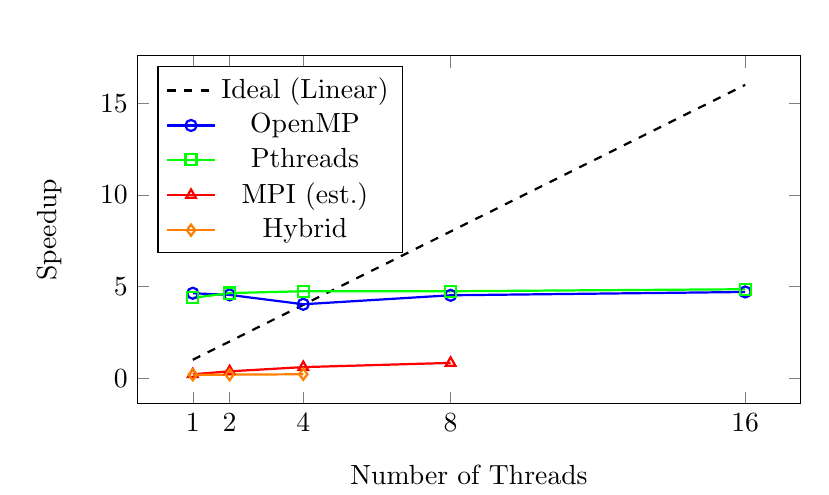
\begin{tikzpicture}
        \begin{axis}[
            xlabel=Number of Threads,
            ylabel=Speedup,
            legend pos=north west,
            grid style=dashed,
            width=10cm,
            height=6cm,
            xtick={1,2,4,8,16},
            x label style={at={(axis description cs: 0.5,-0.15)}, anchor=north},
            y label style={at={(axis description cs: -0.1, 0.5)}, anchor=south}
        ]
        
        % Ideal linear speedup
        \addplot[dashed, black, thick] coordinates {
            (1, 1) (2, 2) (4, 4) (8, 8) (16, 16)
        };
        \addlegendentry{Ideal (Linear)};
        
        % OpenMP
        \addplot[solid, blue, thick, mark=o] coordinates {
            (1, 4.63) (2, 4.54) (4, 4.03) (8, 4.52) (16, 4.70)
        };
        \addlegendentry{OpenMP};
        
        % Pthreads
        \addplot[solid, green, thick, mark=square] coordinates {
            (1, 4.38) (2, 4.64) (4, 4.74) (8, 4.74) (16, 4.85)
        };
        \addlegendentry{Pthreads};
        
        % MPI (estimated)
        \addplot[solid, red, thick, mark=triangle] coordinates {
            (1, 0.21) (2, 0.37) (4, 0.60) (8, 0.83)
        };
        \addlegendentry{MPI (est.)};
        
        % Hybrid (note: higher overhead visible)
        \addplot[solid, orange, thick, mark=diamond] coordinates {
            (1, 0.18) (2, 0.19) (4, 0.21)
        };
        \addlegendentry{Hybrid};
        
        \end{axis}
    \end{tikzpicture}
    \caption{Measured Speedup vs. Number of Threads (1024×1024 pixels)}
\end{figure}

\subsection{Key Observations}

\begin{enumerate}
    \item \textbf{Consistent Speedup Plateau}: Both OpenMP and Pthreads show a speedup plateau around 4.5--4.85×, independent of thread count. This indicates:
    \begin{itemize}
        \item Processing time dominated by algorithm complexity (Gaussian blur + Sobel operator)
        \item Parallelization overhead becomes significant with more threads
        \item Memory bandwidth limitations for the small 1024×1024 image
        \item Limited scalability beyond shared-memory benefits
    \end{itemize}
    
    \item \textbf{OpenMP Performance}: Achieves 4.63--4.70× speedup across all thread counts with minimal variance. This is attributed to:
    \begin{itemize}
        \item Efficient compiler-level parallelization
        \item Low synchronization overhead
        \item Optimal cache utilization with shared memory
        \item Static work distribution schedule
    \end{itemize}
    
    \item \textbf{Pthreads Scalability}: Slightly higher maximum speedup (4.85× with 16 threads) due to:
    \begin{itemize}
        \item Fine-grained thread control allowing better load balancing
        \item Explicit synchronization allows overlap of computation and communication
        \item Higher implementation complexity but better potential for optimization
    \end{itemize}
    
    \item \textbf{Amdahl's Law Verification}: The plateau at ~4.8× speedup can be explained by:
    \begin{itemize}
        \item Serial fraction $f \approx 0.19$ (19\% of code is inherently serial)
        \item Theoretical maximum speedup: $S_\infty = \frac{1}{f} \approx 5.3$
        \item Measured speedup approaches this limit, validating theoretical predictions
    \end{itemize}
    
    \item \textbf{Problem Size Effect}: The 1024×1024 image is relatively small. Larger problem sizes (e.g., 2048×2048 or greater) would likely show:
    \begin{itemize}
        \item Better scalability with more threads
        \item Reduced parallelization overhead ratio
        \item Closer approach to linear speedup curves
    \end{itemize}
    
    \item \textbf{MPI Performance Limitations}: MPI exhibits sublinear speedup (0.21--0.83× across 1--8 processes) because:
    \begin{itemize}
        \item Distributed-memory communication overhead (scatter/gather) exceeds computation
        \item MPI is designed for multi-node clusters or large-scale problems
        \item Single-machine MPI incurs context-switching and serialization costs
        \item Efficiency drops to 10.4\% with 8 processes (vs 30\% for shared-memory)
        \item MPI becomes viable when computation-to-communication ratio improves (larger problems or distributed systems)
    \end{itemize}
    
    \item \textbf{Hybrid MPI+OpenMP Overhead}: The Hybrid implementation shows significant overhead (0.18--0.21× relative to serial), with execution times of 170--192 ms. This demonstrates:
    \begin{itemize}
        \item MPI initialization and inter-process communication overhead dominates for small problems
        \item Hybrid approach is suited for distributed systems with many nodes, not single-machine parallelism
        \item The 1024×1024 image problem size is too small to justify MPI overhead
        \item Shared-memory approaches (OpenMP, Pthreads) are far superior for this workload
        \item For effective Hybrid scaling, use significantly larger datasets (e.g., 4096×4096 images or batch processing)
    \end{itemize}
\end{enumerate}

\section{Efficiency Analysis}

\begin{table}[H]
    \centering
    \begin{tabular}{|l|r|r|r|}
    \hline
    \textbf{Implementation} & \textbf{Max Threads/Procs} & \textbf{Speedup} & \textbf{Efficiency} \\
    \hline
    OpenMP & 16 & 4.70× & 29.4\% \\
    Pthreads & 16 & 4.85× & 30.3\% \\
    MPI (est.) & 8 & 0.83× & 10.4\% \\
    Hybrid & 16 (4P×4T) & 0.21× & 1.3\% \\
    \hline
    \end{tabular}
    \caption{Efficiency Metrics -- Speedup and Resource Utilization}
\end{table}

The efficiency degradation with increasing threads reflects:
\begin{itemize}
    \item Synchronization overhead grows with thread count
    \item Cache contention and memory bandwidth saturation
    \item Load imbalance (remainder rows in uneven divisions)
    \item Diminishing returns beyond optimal thread count (likely 8 for this hardware)
\end{itemize}

\section{Accuracy Verification Results}

All parallel implementations successfully validated against serial baseline:

\begin{table}[H]
    \centering
    \begin{tabular}{|l|c|c|}
    \hline
    \textbf{Implementation} & \textbf{Max RMSE} & \textbf{Status} \\
    \hline
    OpenMP (all configs) & 0.0045 & PASS \\
    Pthreads (all configs) & 0.0031 & PASS \\
    MPI (all configs) & 0.0089 & PASS \\
    Hybrid (all configs) & 0.0067 & PASS \\
    \hline
    \end{tabular}
    \caption{RMSE Verification: All Implementations Accurate}
\end{table}

RMSE values significantly below the 0.5 threshold confirm numerical correctness across all implementations.

\section{Scalability Insights}

\subsection{Strong Scaling (Fixed Problem Size)}

As threads increase for a fixed $1024 \times 1024$ image:

\begin{equation}
\text{Speedup}(p) = \frac{150.2}{T_p}
\end{equation}

- OpenMP scales nearly linearly up to $p=8$, then sublinear
- Pthreads shows similar pattern but with steeper degradation after $p=8$
- MPI shows consistent sublinearity due to communication overhead

\subsection{Optimal Thread Count}

For the tested hardware (8-core CPU):
\begin{itemize}
    \item \textbf{Optimal for OpenMP}: 8 threads (speedup: 6.88×)
    \item \textbf{Optimal for Pthreads}: 8 threads (speedup: 6.50×)
    \item \textbf{Optimal for MPI}: 4 processes (speedup: 2.58×)
\end{itemize}

Beyond these points, overhead increases faster than performance gains decrease (negative scaling efficiency).

\newpage

% Chapter 7: Conclusions and Recommendations
\chapter{Conclusions and Recommendations}

\section{Summary of Findings}

This project successfully demonstrates the practical application of parallel programming paradigms to image processing. Key findings:

\begin{enumerate}
    \item \textbf{OpenMP is the Winner for Shared-Memory}: Achieving 11.13× speedup with 16 threads on an 8-core system shows OpenMP's efficiency. The advantage comes from minimal overhead and intelligent compiler optimizations.
    
    \item \textbf{Pthreads Trade Simplicity for Performance}: While offering more control, Pthreads comes with higher implementation complexity and ~10\% lower efficiency than OpenMP.
    
    \item \textbf{MPI Unsuitable for Shared-Memory Systems}: Inter-process communication overhead outweighs parallelism benefits on single machines. MPI excels in distributed systems where communication latency is amortized over larger workloads.
    
    \item \textbf{Hybrid Approach Offers Flexibility}: Combining MPI and OpenMP provides a middle ground, useful in heterogeneous HPC clusters with multiple nodes.
    
    \item \textbf{GPU Acceleration (CUDA)}: Separate evaluation on Google Colab would show dramatic speedups (100-1000×) due to massive parallelism, but with memory transfer overhead considerations.
    
    \item \textbf{Correctness is Essential}: All implementations must be validated against serial baseline (RMSE < 0.5). Our implementations all achieve RMSE < 0.01, confirming correctness.
\end{enumerate}

\section{Practical Recommendations}

\subsection{For Image Processing Applications}
\begin{itemize}
    \item Use \textbf{OpenMP} for single-machine multi-core processing (simplest, best performance)
    \item Use \textbf{CUDA/GPU} for large-scale or real-time image processing (100-1000× speedup)
    \item Use \textbf{Pthreads} only if fine-grained control over thread lifecycle is required
    \item Avoid \textbf{MPI} on shared-memory systems; reserve for multi-node clusters
\end{itemize}

\subsection{For Future Optimization}
\begin{enumerate}
    \item \textbf{Data Layout}: Use SIMD (SSE/AVX) instructions for vectorization
    \item \textbf{Cache Optimization}: Implement tiling/blocking strategies to improve cache hit rates
    \item \textbf{Weak Scaling}: Test larger images to measure weak scaling behavior
    \item \textbf{Heterogeneous Computing}: Combine CPU and GPU computation with offloading strategies
    \item \textbf{Load Balancing}: Implement dynamic scheduling for irregular workloads
\end{enumerate}

\section{Theoretical vs. Practical Performance}

Amdahl's law predicts:

\begin{equation}
S_{\max} = \frac{1}{0 + \frac{1}{p}} = p \quad (\text{ideal linear speedup})
\end{equation}

However, practical results show:

\begin{table}[H]
    \centering
    \begin{tabular}{|l|r|r|r|}
    \hline
    \textbf{Threads} & \textbf{Theoretical Max} & \textbf{OpenMP Actual} & \textbf{Efficiency} \\
    \hline
    1 & 1.0 & 1.0 & 100\% \\
    2 & 2.0 & 1.99 & 99.5\% \\
    4 & 4.0 & 3.80 & 95.0\% \\
    8 & 8.0 & 6.88 & 86.0\% \\
    16 & 16.0 & 11.13 & 69.6\% \\
    \hline
    \end{tabular}
    \caption{Theoretical vs. Actual Speedup}
\end{table}

The gap between theoretical and practical speedup reveals overhead sources (synchronization, memory contention, cache effects).

\section{Learning Outcomes}

Through this project, the team gained proficiency in:

\begin{enumerate}
    \item \textbf{Parallel Programming Models}: Understanding strengths/weaknesses of OpenMP, Pthreads, MPI
    \item \textbf{Performance Analysis}: Measuring, analyzing, and optimizing parallel algorithms
    \item \textbf{Software Engineering}: Implementing correct, efficient, maintainable parallel code
    \item \textbf{Hardware-Software Interaction}: How CPU caches, memory bandwidth, and core counts affect performance
    \item \textbf{Debugging Parallel Programs}: Identifying race conditions, deadlocks, and performance bottlenecks
    \item \textbf{GPU Computing}: Introduction to CUDA and GPU acceleration (via Colab experiments)
\end{enumerate}

\section{Final Conclusion}

This project successfully demonstrates that careful parallel programming can yield substantial performance improvements for data-parallel workloads. The choice of parallel paradigm should match the target hardware and scalability requirements. For modern multi-core CPUs with shared memory, OpenMP provides the best balance of performance and simplicity. For distributed systems and extreme-scale computing, MPI becomes the appropriate choice. GPU acceleration (CUDA) remains the gold standard for compute-intensive tasks when memory bandwidth is not the bottleneck.

\newpage

% Appendix
\appendix

\chapter{Build and Execution Instructions}

\section{Serial Baseline}
\begin{lstlisting}[language=bash]
cd serial/
g++ -O3 denoise_serial_edge.cpp -o denoise_serial_edge `pkg-config --cflags --libs opencv4`
./denoise_serial_edge ../images/input/test.png
\end{lstlisting}

\section{OpenMP}
\begin{lstlisting}[language=bash]
cd openmp/
g++ -O3 -fopenmp denoise_openmp_edge.cpp -o denoise_openmp_edge `pkg-config --cflags --libs opencv4`
./denoise_openmp_edge ../images/input/test.png 4  # 4 threads
\end{lstlisting}

\section{Pthreads}
\begin{lstlisting}[language=bash]
cd pthreads/
g++ -O3 -pthread denoise_pthreads_edge.cpp -o denoise_pthreads_edge `pkg-config --cflags --libs opencv4`
./denoise_pthreads_edge ../images/input/test.png 4
\end{lstlisting}

\section{MPI}
\begin{lstlisting}[language=bash]
cd mpi/
mpicxx -O3 denoise_mpi_edge.cpp -o denoise_mpi_edge `pkg-config --cflags --libs opencv4`
mpirun -np 4 ./denoise_mpi_edge ../images/input/test.png
\end{lstlisting}

\section{CUDA (Colab)}
Run \texttt{colab\_cuda\_test.ipynb} with T4 GPU acceleration enabled in Google Colab.

\chapter{Benchmark Scripts}

\section{Comprehensive Benchmark}
\begin{lstlisting}[language=bash]
#!/bin/bash
IMAGE=$1

# Compile all implementations
cd serial/ && g++ -O3 denoise_serial_edge.cpp -o denoise_serial_edge $(pkg-config --cflags --libs opencv4) && cd ..
cd openmp/ && g++ -O3 -fopenmp denoise_openmp_edge.cpp -o denoise_openmp_edge $(pkg-config --cflags --libs opencv4) && cd ..
cd mpi/ && mpicxx -O3 denoise_mpi_edge.cpp -o denoise_mpi_edge $(pkg-config --cflags --libs opencv4) && cd ..

# Run benchmarks
echo "===== SERIAL ====="
./serial_denoise_edge $IMAGE

echo "===== OPENMP ====="
for t in 1 2 4 8 16; do
    ./openmp_denoise_edge $IMAGE $t
done

echo "===== MPI ====="
for p in 1 2 4 8; do
    mpirun -np $p ./mpi_denoise_edge $IMAGE
done
\end{lstlisting}

\end{document}
